\documentclass[11pt, a4paper]{article}

\usepackage[utf8]{inputenc}
\usepackage[T1]{fontenc}
\usepackage{amsmath}
\usepackage{amssymb}
\usepackage{graphicx}
\usepackage{geometry}
\usepackage{fancyhdr}
\usepackage{enumitem}
\usepackage{array}
\usepackage{eso-pic}
\usepackage{esvect}
\usepackage{tikz}
\usetikzlibrary{arrows.meta,calc}
\usepackage[most]{tcolorbox}

\usepackage{siunitx}
\DeclareSIUnit{\litre}{l}
\sisetup{
    locale = DE,
    inter-unit-product = \cdot,
    per-mode = symbol-or-fraction
}

\makeatletter
\def\input@path{{./}{../../}}
\makeatother

\geometry{a4paper, top=2.5cm, bottom=2.5cm, left=2.5cm, right=2.5cm}

\input{defs}

% --- Lösungsbox-Umgebung ---
\definecolor{boxcol_back_lgreen}{RGB}{220, 255, 220}
\definecolor{boxcol_back_white}{RGB}{255, 255, 255}
\definecolor{boxcol_frame_green}{RGB}{30, 180, 30}
\newtcolorbox{solutionbox}[1][] {
  colback=boxcol_back_white,
  colframe=boxcol_frame_green,
  colbacktitle=boxcol_back_lgreen,
  fonttitle=\bfseries,
  coltitle=black,
  boxsep=5pt,
  arc=1mm,
  enhanced,
  attach boxed title to top left={yshift=-2mm, xshift=3mm},
  title=Lösung,
  #1
}
% ---

\pagestyle{fancy}
\fancyhf{}
\cfoot{\thepage}

\begin{document}

\section*{\LARGE Lösung: Kurztest 3}
\noindent
\begin{tabular}{ll}
    \textbf{Gruppe: } & \LARGE\textbf{A}  \\[0.3cm]
\end{tabular}

\begin{enumerate}[label=\textbf{\arabic*.},itemsep=0.50cm]

    \item (1,5 P) - \textbf{Newtonsche Axiome:} \\
    Geben Sie die drei Newtonschen Axiome an und erläutern Sie kurz, was jedes Axiom besagt.
    \begin{solutionbox}
        \begin{itemize}[itemsep=0pt, topsep=0pt]
            \item \textbf{1. Newtonsches Axiom (Trägheitssatz):} Ein Körper bleibt in Ruhe oder in gleichförmiger geradliniger Bewegung, solange keine resultierende Kraft auf ihn wirkt.
            \item \textbf{2. Newtonsches Axiom:} Wirkt auf einen Körper eine resultierende Kraft, so erfährt er eine Beschleunigung. Es gilt $\vec{F}_{\mathrm{res}} = m \cdot \vec{a}$.
            \item \textbf{3. Newtonsches Axiom (Actio gleich Reactio):} Kräfte treten immer paarweise auf. Übt ein Körper A auf B eine Kraft aus, so übt B auf A eine gleich große, entgegengesetzt gerichtete Kraft aus.
        \end{itemize}
    \end{solutionbox}

    \item (1,5 P) - \textbf{Kraft aus Beschleunigung:} \\
    Es wirken die folgenden drei Kräfte auf einen Körper der Masse $m = 2\, \text{kg}$:
    \begin{equation*}
        \vec{F}_1 = \begin{pmatrix} 3 \\ 0 \\ -1 \end{pmatrix} \, \text{N}, \quad \vec{F}_2 = \begin{pmatrix} 0 \\ 4 \\ 2 \end{pmatrix} \, \text{N}, \quad \vec{F}_3 = \begin{pmatrix} -5 \\ 2 \\ 7 \end{pmatrix} \, \text{N}
    \end{equation*}
    Berechne die resultierende Kraft $\vec{F}_{\text{res}}$ und die Beschleunigung $\vec{a}$ des Körpers.
    \begin{solutionbox}
        Zuerst die resultierende Kraft:
        \[
        \vec{F}_{\text{res}} = \vec{F}_1 + \vec{F}_2 + \vec{F}_3
        = \begin{pmatrix} 3 \\ 0 \\ -1 \end{pmatrix} + \begin{pmatrix} 0 \\ 4 \\ 2 \end{pmatrix} + \begin{pmatrix} -5 \\ 2 \\ 7 \end{pmatrix}
        = \begin{pmatrix} -2 \\ 6 \\ 8 \end{pmatrix} \, \text{N}
        \]
        Mit dem 2. Newtonschen Axiom folgt
        \[
        \vec{a} = \frac{\vec{F}_{\text{res}}}{m} = \frac{1}{2} \begin{pmatrix} -2 \\ 6 \\ 8 \end{pmatrix}
        = \begin{pmatrix} -1 \\ 3 \\ 4 \end{pmatrix} \, \si{\meter\per\second\squared}
        \]
    \end{solutionbox}

    \item (2 P) - \textbf{Reibung auf der schiefen Ebene:} \\
    Ein Körper der Masse $m = 5\, \text{kg}$ liegt auf einer schiefen Ebene, die einen Winkel von $\alpha = 30^\circ$ zur Horizontalen bildet. Der Haftreibungskoeffizient beträgt $\mu_H = \SI{0.4}{}$. Wird der Körper auf der schiefen Ebene gehalten oder beginnt er zu rutschen? Berechnen Sie dazu die Hangabtriebskraft $F_A$ und die maximale Haftreibungskraft $F_{R,h,\text{max}}$.
    \begin{solutionbox}
        Mit $g = \SI{10}{\meter\per\second\squared}$ gilt:
        Die Hangabtriebskraft lautet
        \[
        F_A = m g \sin\alpha = 5 \cdot 10 \cdot \sin 30^\circ = \SI{25}{\newton}
        \]
        Die maximale Haftreibungskraft ist
        \[
        F_{R,h,\text{max}} = \mu_H \cdot m g \cos\alpha = \num{0.4} \cdot 5 \cdot 10 \cdot \cos 30^\circ \approx \SI{17.3}{\newton}
        \]
        Da $F_A > F_{R,h,\text{max}}$, reicht die Haftreibung nicht aus. Der Körper beginnt daher, die Ebene hinunterzurutschen.

        \begin{center}
        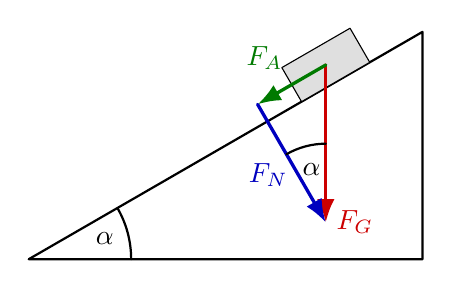
\begin{tikzpicture}[scale=1.0, >=Latex, line cap=round, line join=round]
            \coordinate (A) at (0,0);
            \coordinate (B) at (5,0);
            \coordinate (C) at (5,2.88675);
            \coordinate (P) at ($(A)+(30:4)$);
            \coordinate (M) at ($(P)+(30:0.5)+(120:0.25)$);
            \coordinate (Gend) at ($(M)+(0,-2)$);
            \coordinate (Aend) at ($(M)+(210:1.)$);

            \draw[thick] (A) -- (B) -- (C) -- (A);

            \draw[fill=gray!25, rotate around={30:(P)}] ($(P)$) rectangle ($(P)+(1,0.5)$);

            \draw[->, very thick, red!80!black] (M) -- (Gend) node[right] {$F_G$};
            \draw[->, very thick, blue!75!black] (Aend) -- (Gend) node[pos=0.6, left] {$F_N$};
            \draw[->, very thick, green!60!black!80!black] (M) -- (Aend) node[pos=0.9, above=0.25cm] {$F_A$};

            \draw[thick] ($(A)+(1.3,0)$) arc[start angle=0,end angle=30,radius=1.3];
            \node at ($(A)+(15:1.0)$) {$\alpha$};
            \draw[thick] ($(Gend)+(0,1)$) arc[start angle=90,end angle=120,radius=1.];
            \node at ($(Gend)+(105:0.7)$) {$\alpha$};

        \end{tikzpicture}
        \end{center}
    \end{solutionbox}

    \item (1 P) - \textbf{Federkraft:} \\
    Eine Feder hat eine Federkonstante von $k = \SI{150}{\newton\per\meter}$. Welche Kraft wirkt auf die Feder (achten Sie auf das Vorzeichen), wenn sie um $\Delta x = \SI{0.2}{\meter}$ bzw. $\Delta x = \SI{-1}{\meter}$ gedehnt wird?
    \begin{solutionbox}
        Nach dem Hookeschen Gesetz gilt
        \[
        F = -k \Delta x
        \]
        Für $\Delta x = \SI{0.2}{\meter}$ ergibt sich
        \[
        F = -150 \cdot \num{0.2} = \SI{-30}{\newton}
        \]
        Für $\Delta x = \SI{-1}{\meter}$ folgt
        \[
        F = -150 \cdot \num{-1} = \SI{150}{\newton}
        \]
    \end{solutionbox}

    \item (1 P) - \textbf{Feder-Masse-System:} \\
    An einer Feder mit $k = \SI{200}{\newton\per\meter}$ hängt eine Masse von \SI{2}{\kilogram} im Gleichgewicht. Wie groß ist die Dehnung der Feder?
    \begin{solutionbox}
        Im Gleichgewicht gilt
        \[
        kx = mg
        \]
        also
        \[
        x = \frac{mg}{k} = \frac{2 \cdot 10}{200} = \SI{0.1}{\meter}
        \]
        Die Feder dehnt sich also um \SI{10}{\centi\meter}.
    \end{solutionbox}

    \item (1,5 P) - \textbf{Geschwindigkeit des Körpers im Hookeschen Gesetz} \\
    Sie möchten eine Formel für die Geschwindigkeit eines Körpers mit Masse $m$ bestimmen, der an einer Feder mit Federkonstante $k$ hängt. Zeigen Sie, dass das unweigerlich auf die Gleichung
    \begin{equation*}
        m \cdot v \cdot \mathrm{d}v = -k \cdot x \cdot \mathrm{d}x
    \end{equation*}
    hinausläuft, wobei $x$ die Auslenkung der Feder von der Ruhelage ist. \\
    \textit{Tipp: }Ersetzen Sie im Hookeschen Gesetz die Kraft $F$ mithilfe des 2. Newtonschen Axioms. Anschließend verwenden Sie die Kettenregel $\cfrac{da}{dc} = \cfrac{da}{db} \, \cfrac{db}{dc}$.
    \begin{solutionbox}
        Mit dem Hookeschen Gesetz und dem 2. Newtonschen Axiom gilt
        \[
        F = -kx \quad \text{und} \quad F = m a = m \frac{\mathrm{d}v}{\mathrm{d}t}
        \]
        Also
        \[
        m \frac{\mathrm{d}v}{\mathrm{d}t} = -kx
        \]
        Mit der Kettenregel
        \[
        \frac{\mathrm{d}v}{\mathrm{d}t} = \frac{\mathrm{d}v}{\mathrm{d}x} \cdot \frac{\mathrm{d}x}{\mathrm{d}t} = v \frac{\mathrm{d}v}{\mathrm{d}x}
        \]
        folgt
        \[
        m v \frac{\mathrm{d}v}{\mathrm{d}x} = -kx
        \]
        und nach Multiplikation mit $\mathrm{d}x$ erhält man
        \[
        m \cdot v \cdot \mathrm{d}v = -k \cdot x \cdot \mathrm{d}x
        \]
    \end{solutionbox}

    \item (1,5 P) - \textbf{Integration der Geschwindigkeit:} \\
    In der vorherigen Aufgabe haben Sie die Gleichung
    \begin{equation*}
        m \cdot v \cdot \mathrm{d}v = -k \cdot x \cdot \mathrm{d}x
    \end{equation*}
    hergeleitet. Integrieren Sie diese Gleichung, um eine Formel für die Geschwindigkeit $v$ in Abhängigkeit von der Auslenkung $x$ zu erhalten. Nehmen Sie an, dass die Geschwindigkeit $v = 0$ ist, wenn die Auslenkung $x = A$ (die maximale Auslenkung) beträgt.
    \begin{solutionbox}
        Integration mit den Grenzen $v: 0 \to v$ und $x: A \to x$:
        \[
        \int_0^v m v \, \mathrm{d}v = -\int_A^x k x \, \mathrm{d}x
        \]
        Daraus folgt
        \[
        \frac{1}{2} m v^2 = \frac{1}{2} k \left(A^2 - x^2\right)
        \]
        und damit
        \[
        v = \sqrt{\frac{k}{m}\left(A^2 - x^2\right)}
        \]
        Für die Geschwindigkeit als Betrag ist die positive Wurzel gemeint.
    \end{solutionbox}

\end{enumerate}

\vspace{1cm}

\end{document}